%!TEX root = ../main.tex
For the internal segmentation we have adapted the binary segmentation algorithm (BSA) \cite{lee2012binary}. This algorithm aims to segment an image into two sub-images on the segmentation point that is most likely. One of these sub images is then selected and segmented again into two new sub-images. Which sub-image is selected for further segmentation depends on the selection criterion. \Cref{fig:method:segmentation:overview} gives a schematic overview of this process. \Cref{sss:method:segmentation:parameterEstimation} discuss the parameters that are determined based on the lexicon and the word image. The following sections, \cref{sss:method:segmentation:sspGeneration,sss:method:segmentation:subImageSelection,sss:method:segmentation:binarySegmentation,sss:method:segmentation:terminatingCondition}, discuss several of the modules used in \cref{fig:method:segmentation:overview}.

\begin{figure}
	\centering
	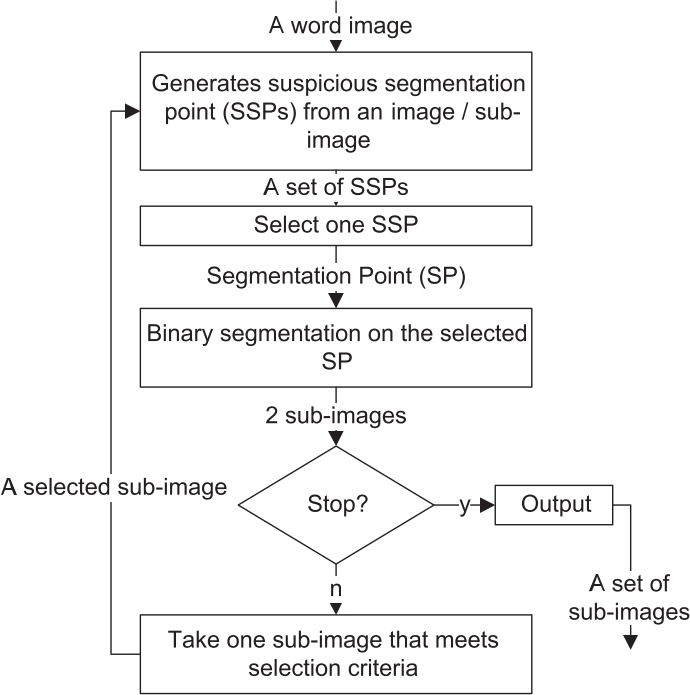
\includegraphics[width=\columnwidth]{shared/img/method/segmentation_pipeline.png}
	\caption{The internal segmentation pipeline, image from \cite{lee2012binary}.}
	\label{fig:method:segmentation:overview}
\end{figure}

\subsubsection{Parameter Estimation}
	\label{sss:method:segmentation:parameterEstimation}
	Several parameters need to be set for this algorithm: the segmentation criterion, the minimum character width, the average character width and the maximum number of segmentations. These parameters are all based on either, the word image, the lexicon or the train data.

	% Stroke Width: 2.3.1
	The stroke width (\texttt{SW}) refers to how thick the stroke of a pen is. We compute the stroke width as the mode of the number of sequential foreground pixels in one row or column of pixels in the horizontal and the vertical direction respectively. Stroke width is used in the generation of suspicious segmentation points including avoiding under-segmentations.

	%Baseline: 2.3.2
	The baseline of the word is computed as the row with the most foreground pixels. \Cref{fig:method:segmentation:baselinecomputation} shows an example of the result of this baseline computation. The baseline is used to reduce the influence of extensive ligatures in cursive handwriting when generation suspicious segmentation points, among other things.

	% ACW and MCW
	The average character width (\texttt{ACW}), minimum character width (\texttt{MCW}), minimum character height (\texttt{MCW}) and the minimum number of foreground pixels (\texttt{MFP}) are computed based on the training data.

	\begin{figure}
		\laura{For the final version show both the histogram and the computed baselines in one image.}
		\centering
		
\includegraphics[width=\columnwidth]{shared/img/method/baseline_computation.jpg}
		\caption{An example of the computed baselines.}
		\label{fig:method:segmentation:baselinecomputation}
	\end{figure}

	%Maximum number of segmentations
	The maximum number of segmentations (\texttt{MNS}) is set to the number of characters of the longest word in the lexicon. This value is used to determine the maximum sub images one should extract from one word. 

\subsubsection{Suspicious Segmentation Points Generation}
	\label{sss:method:segmentation:sspGeneration}
	%2.3
	The suspicious segmentation point generation module receives an image, either a word image or a sub image, and produces a set of suspicious segmentation points. 

	This process only looks at pixels between baselines, to minimize the influence of of extensive ligatures. A column of pixels in the image is only considered as a possible suspicious segmentation point if its vertical pixel density is greater than $2 \cdot \mathtt{SW}$. This threshold results in a set of possible suspicious segmentation points. From this set all suspicious regions, a group of continuous possible suspicious segmentation points, is extracted. If the width of a suspicious region is less than \texttt{SW}, a suspicious segmentation point is placed in the middle of the suspicious region. Suspicious segmentation points are placed at the start and the end of the suspicious region and at intervals of \texttt{SW} within the region, see the example in \cref{fig:method:segmentation:suspiciousSegmentationPoints}.

	\begin{figure}
		\timemachine{Create this image based on our dataset ourselves.}
		\centering
		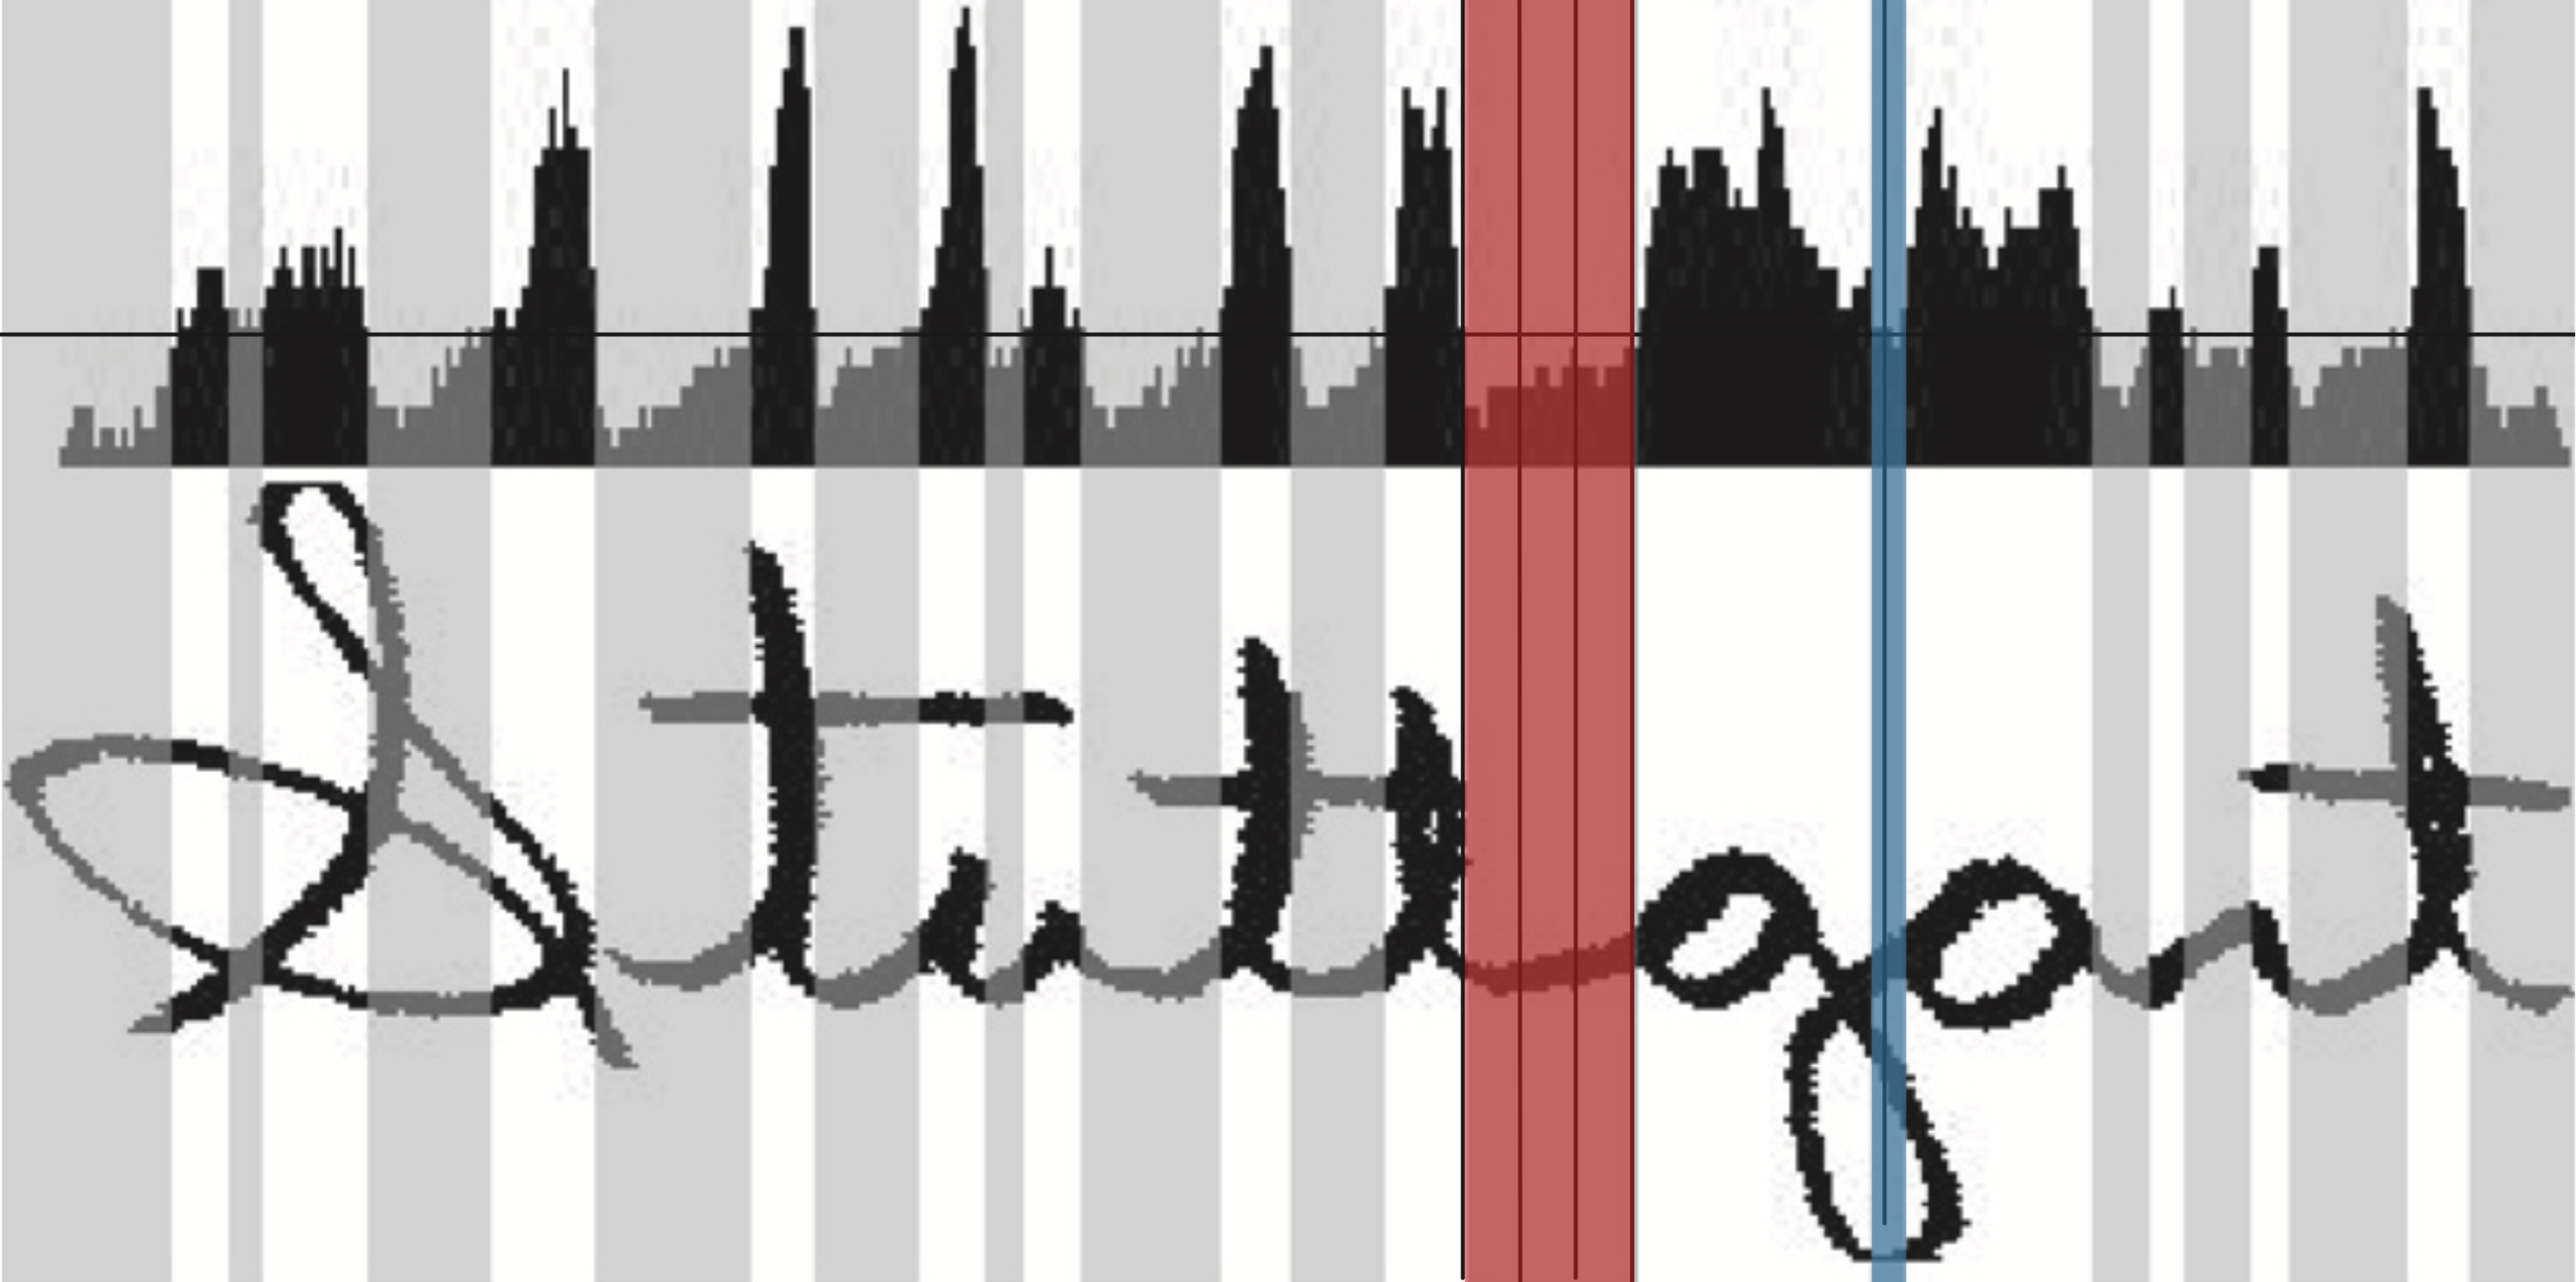
\includegraphics[width=\columnwidth]{shared/img/method/suspicious_regions.png}
		\caption{An image of a word, and the vertical pixel density histogram of the body region, the are between the baselines, of that word. The threshold for suspicious regions is shown as a line in the histogram. The shaded areas show the suspicious regions. For the two red shaded regions the suspiciosus segmentations points are drawn. The image is adapted from \cite{lee2012binary}.}
		\label{fig:method:segmentation:suspiciousSegmentationPoints}
	\end{figure}

	This set of suspicious segmentation points is then filtered based by removing all suspicious segmentation points that are located in the hole of a letter. Holes are detected via region growing algorithm. Region growing algorithms require as input an image array $f(x,y)$, a seed array $s(x,y)$ of the same size as $f(x,y)$ and a predicate that is to be applied to one pixel. The seed array contains all suspicious segmentation points. Connected components in $s(x,y)$ are eroded to one pixel. A binary image $f_Q(x,y)$ is formed, such that
	\begin{equation*}
		f_Q(x,y) = 
		\begin{cases}
			1 & \text{if }Q(f(x,y)) = 1,\\
			0 & \text{otherwise.}
		\end{cases}
	\end{equation*}
	The final image $g$ is formed by appending to each seed point all the 1-valued points in $f_Q$ that are eight connected to the seed point \cite{gonzalez2002digitalCh10}. All connected components in $g$ that do not reach the boundary of the image are considered holes. This process is illustrated for one letter in \cref{fig:method:segmentation:holeDetection}. This example also shows a problem with this algorithm, namely that holes that are not completely closed are not seen as holes. 

		\begin{figure}
		\centering
		\subfloat[]{
			
\includegraphics[width=0.23\linewidth]{shared/img/method/hole_detection_fxy.png}%
			\label{fig:method:segmentation:holeDetection:fxy}%
		}
		\hfil
		\subfloat[]{
			
\includegraphics[width=0.23\linewidth]{shared/img/method/hole_detection_sxy.png}%
			\label{fig:method:segmentation:holeDetection:seed}%
		}
		\hfil
		\subfloat[]{
			
\includegraphics[width=0.23\linewidth]{shared/img/method/hole_detection_fqxy.png}%
			\label{fig:method:segmentation:holeDetection:fqxy}%
		}
		\hfil
		\subfloat[]{
			
\includegraphics[width=0.23\linewidth]{shared/img/method/hole_detection_g.png}%
			\label{fig:method:segmentation:holeDetection:g}%
		}				
		\caption{An example of hole detection on \protect\subref{fig:method:segmentation:holeDetection:fxy} the image array $f(x,y)$ representing the letter `b', with \protect\subref{fig:method:segmentation:holeDetection:seed} the seed array $s(x,y)$ which contains the suspicious segmentation points. Filtering the \protect\subref{fig:method:segmentation:holeDetection:fqxy} connected components, that were found after applying predicate $Q$ to $f(x,y)$ results in \protect\subref{fig:method:segmentation:holeDetection:g} one of the holes of the letter.}
		\label{fig:method:segmentation:holeDetection}
	\end{figure}

\subsubsection{Binary Segmentation}
	\label{sss:method:segmentation:binarySegmentation}
	Given a segmentation point, defined as some x-coordinate in the image, this module tries to split the image into two sub-images. 

	In optical character recognition this is generally done by cutting the image in two along a vertical line through the segmentation point. This is not effective in the recognition of handwriting for a plethora of reasons. One of them is the lack of guarantee that there are spaces between characters \cite{lee2012binary}. Instead we trace the foreground pixel contour, we start on the lowest row of pixels in the word image, at the segmentation point and trace the neighboring background pixels to avoid cutting foreground pixels until we reach the highest row of pixels in the word image. If no path of continuous background pixels can be traced then foreground pixels may only be cut if they are on vertical line defined by the segmentation point. 

	After binary segmentation the new sub-images should should have a width and height that is greater than \texttt{MCW} and \texttt{MCH} respectively. Furthermore both sub-images should have a more foreground pixels than \texttt{MFP}. If the images do not satisfy these conditions they are discarded, as is the suspicious segmentation point that they resulted from. 

\subsubsection{Terminating Condition}
	\label{sss:method:segmentation:terminatingCondition}
	%2.2
	The terminating condition is based on the size of the sub-images and the number of sub-images. To avoid infinite loops it is also required that at least on sub-image can be over-segmented to generate suspicious segmentation points. If no more sub-images can be over segmented the algorithm terminates. The size requirement states that each sub-image should have a width that is in the range $[\mathtt{MCW}, \mathtt{MCW} + \mathtt{ACW}]$. The cardinality requirement asserts that the number of generated sub-images should be smaller than \texttt{MNS}.

\subsubsection{Sub-Image Selection}
	\label{sss:method:segmentation:subImageSelection}
	%2.1
	Sub image selection selects the next sub-image to be separated into two new subimages.

	In general a sub image is selected for further segmentation from the set of sub-images if it has suspicious segmentation points and its width is greater than the average character width. If multiple sub-images satisfy these conditions the image with the greatest width is chosen. To ensure that non-connected overlapping characters are segmented first sub-images that are separable by space between characters are segmented through that space, regardless of the suspicious segmentation points.